% -*- Mode:TeX -*-

%% IMPORTANT: The official thesis specifications are available at:
%%            http://libraries.mit.edu/archives/thesis-specs/
%%
%%            Please verify your thesis' formatting and copyright
%%            assignment before submission. If you notice any
%%            discrepancies between these templates and the 
%%            MIT Libraries' specs, please let us know
%%            by e-mailing thesis@mit.edu

%% The documentclass options along with the pagestyle can be used to generate
%% a technical report, a draft copy, or a regular thesis. You may need to
%% re-specify the pagestyle after you \include cover.tex. For more
%% information, see the first few lines of mitthesis.cls. 

%\documentclass[12pt,vi,twoside]{mitthesis}
%%
%%  If you want your thesis copyright to you instead of MIT, use the
%%  ``vi'' option, as above.
%%
%\documentclass[12pt,twoside,leftblank]{mitthesis}
%%
%% If you want blank pages before new chapters to be labelled ``This
%% Page Intentionally Left Blank'', use the ``leftblank'' option, as
%% above. 

\documentclass[11pt,twoside]{mitthesis}
\usepackage{lgrind}
%% These have been added at the request of the MIT Libraries, because
%% some PDF conversions mess up the ligatures.  -LB, 1/22/2014
\usepackage{cmap}
\usepackage{graphicx}
\usepackage{subfig}
\usepackage{amsmath}
\usepackage[T1]{fontenc}
\pagestyle{plain}

%% This bit allows you to either specify only the files which you wish to
%% process, or `all' to process all files which you \include.
%% Krishna Sethuraman (1990).

%\typein [\files]{Enter file names to process, (chap1,chap2 ...), or `all' to process all files:}
\def\all{all}
\ifx\files\all \typeout{Including all files.} \else %\typeout{Including only \files.} \includeonly{\files} \fi

\begin{document}

% -*-latex-*-
% 
% For questions, comments, concerns or complaints:
% thesis@mit.edu
% 
%
% $Log: cover.tex,v $
% Revision 1.9  2019/08/06 14:18:15  cmalin
% Replaced sample content with non-specific text.
%
% Revision 1.8  2008/05/13 15:02:15  jdreed
% Degree month is June, not May.  Added note about prevdegrees.
% Arthur Smith's title updated
%
% Revision 1.7  2001/02/08 18:53:16  boojum
% changed some \newpages to \cleardoublepages
%
% Revision 1.6  1999/10/21 14:49:31  boojum
% changed comment referring to documentstyle
%
% Revision 1.5  1999/10/21 14:39:04  boojum
% *** empty log message ***
%
% Revision 1.4  1997/04/18  17:54:10  othomas
% added page numbers on abstract and cover, and made 1 abstract
% page the default rather than 2.  (anne hunter tells me this
% is the new institute standard.)
%
% Revision 1.4  1997/04/18  17:54:10  othomas
% added page numbers on abstract and cover, and made 1 abstract
% page the default rather than 2.  (anne hunter tells me this
% is the new institute standard.)
%
% Revision 1.3  93/05/17  17:06:29  starflt
% Added acknowledgements section (suggested by tompalka)
% 
% Revision 1.2  92/04/22  13:13:13  epeisach
% Fixes for 1991 course 6 requirements
% Phrase "and to grant others the right to do so" has been added to 
% permission clause
% Second copy of abstract is not counted as separate pages so numbering works
% out
% 
% Revision 1.1  92/04/22  13:08:20  epeisach

% NOTE:
% These templates make an effort to conform to the MIT Thesis specifications,
% however the specifications can change. We recommend that you verify the
% layout of your title page with your thesis advisor and/or the MIT 
% Libraries before printing your final copy.
\title{MIT Thesis Template in Overleaf}

\author{Tim Beaver}
% If you wish to list your previous degrees on the cover page, use the 
% previous degrees command:
%       \prevdegrees{A.A., Harvard University (1985)}
% You can use the \\ command to list multiple previous degrees
%       \prevdegrees{B.S., University of California (1978) \\
%                    S.M., Massachusetts Institute of Technology (1981)}
\department{Department of Electrical Engineering and Computer Science}

% If the thesis is for two degrees simultaneously, list them both
% separated by \and like this:
% \degree{Doctor of Philosophy \and Master of Science}
\degree{Bachelor of Science in Computer Science and Engineering}

% As of the 2007-08 academic year, valid degree months are September, 
% February, or June.  The default is June.
\degreemonth{June}
\degreeyear{1990}
\thesisdate{May 18, 1990}

%% By default, the thesis will be copyrighted to MIT.  If you need to copyright
%% the thesis to yourself, just specify the `vi' documentclass option.  If for
%% some reason you want to exactly specify the copyright notice text, you can
%% use the \copyrightnoticetext command.  
%\copyrightnoticetext{\copyright IBM, 1990.  Do not open till Xmas.}

% If there is more than one supervisor, use the \supervisor command
% once for each.
\supervisor{William J. Supervisor}{Associate Professor}

% This is the department committee chairman, not the thesis committee
% chairman.  You should replace this with your Department's Committee
% Chairman.
\chairman{Arthur C. Chairman}{Chairman, Department Committee on Graduate Theses}

% Make the titlepage based on the above information.  If you need
% something special and can't use the standard form, you can specify
% the exact text of the titlepage yourself.  Put it in a titlepage
% environment and leave blank lines where you want vertical space.
% The spaces will be adjusted to fill the entire page.  The dotted
% lines for the signatures are made with the \signature command.
\maketitle

% The abstractpage environment sets up everything on the page except
% the text itself.  The title and other header material are put at the
% top of the page, and the supervisors are listed at the bottom.  A
% new page is begun both before and after.  Of course, an abstract may
% be more than one page itself.  If you need more control over the
% format of the page, you can use the abstract environment, which puts
% the word "Abstract" at the beginning and single spaces its text.

%% You can either \input (*not* \include) your abstract file, or you can put
%% the text of the abstract directly between the \begin{abstractpage} and
%% \end{abstractpage} commands.

% First copy: start a new page, and save the page number.
%\cleardoublepage
% Uncomment the next line if you do NOT want a page number on your
% abstract and acknowledgments pages.
% \pagestyle{empty}
\setcounter{savepage}{\thepage}
\begin{abstractpage}
% $Log: abstract.tex,v $
% Revision 1.1  93/05/14  14:56:25  starflt
% Initial revision
% 
% Revision 1.1  90/05/04  10:41:01  lwvanels
% Initial revision
% 
%
%% The text of your abstract and nothing else (other than comments) goes here.
%% It will be single-spaced and the rest of the text that is supposed to go on
%% the abstract page will be generated by the abstractpage environment.  This
%% file should be \input (not \include 'd) from cover.tex.
Lorem ipsum dolor sit amet, consectetur adipiscing elit. Nam quis neque et erat laoreet finibus at ac leo. Curabitur pellentesque, diam quis dignissim finibus, enim dui feugiat leo, nec porttitor sapien mi ac felis. Nam aliquam pretium nibh, quis dapibus dolor gravida sit amet. Cras porttitor dui quis elementum pulvinar. Nulla id pulvinar massa. Nullam ut diam non lorem venenatis faucibus. Vivamus lacus ante, pellentesque vitae nisl sit amet, bibendum facilisis purus.

\end{abstractpage}

% Additional copy: start a new page, and reset the page number.  This way,
% the second copy of the abstract is not counted as separate pages.
% Uncomment the next 6 lines if you need two copies of the abstract
% page.
% \setcounter{page}{\thesavepage}
% \begin{abstractpage}
% % $Log: abstract.tex,v $
% Revision 1.1  93/05/14  14:56:25  starflt
% Initial revision
% 
% Revision 1.1  90/05/04  10:41:01  lwvanels
% Initial revision
% 
%
%% The text of your abstract and nothing else (other than comments) goes here.
%% It will be single-spaced and the rest of the text that is supposed to go on
%% the abstract page will be generated by the abstractpage environment.  This
%% file should be \input (not \include 'd) from cover.tex.
Lorem ipsum dolor sit amet, consectetur adipiscing elit. Nam quis neque et erat laoreet finibus at ac leo. Curabitur pellentesque, diam quis dignissim finibus, enim dui feugiat leo, nec porttitor sapien mi ac felis. Nam aliquam pretium nibh, quis dapibus dolor gravida sit amet. Cras porttitor dui quis elementum pulvinar. Nulla id pulvinar massa. Nullam ut diam non lorem venenatis faucibus. Vivamus lacus ante, pellentesque vitae nisl sit amet, bibendum facilisis purus.

% \end{abstractpage}

%\cleardoublepage

% \section*{Acknowledgments}

% This is the acknowledgements section. You should replace this with your
% own acknowledgements.

%%%%%%%%%%%%%%%%%%%%%%%%%%%%%%%%%%%%%%%%%%%%%%%%%%%%%%%%%%%%%%%%%%%%%%
% -*-latex-*-

% Some departments (e.g. 5) require an additional signature page.  See
% signature.tex for more information and uncomment the following line if
% applicable.
% % -*- Mode:TeX -*-
%
% Some departments (e.g. Chemistry) require an additional cover page
% with signatures of the thesis committee.  Please check with your
% thesis advisor or other appropriate person to determine if such a 
% page is required for your thesis.  
%
% If you choose not to use the "titlepage" environment, a \newpage
% commands, and several \vspace{\fill} commands may be necessary to
% achieve the required spacing.  The \signature command is defined in
% the "mitthesis" class
%
% The following sample appears courtesy of Ben Kaduk <kaduk@mit.edu> and
% was used in his June 2012 doctoral thesis in Chemistry. 

\begin{titlepage}
\begin{large}
This doctoral thesis has been examined by a Committee of the Department
of Chemistry as follows:

\signature{Professor Jianshu Cao}{Chairman, Thesis Committee \\
   Professor of Chemistry}

\signature{Professor Troy Van Voorhis}{Thesis Supervisor \\
   Associate Professor of Chemistry}

\signature{Professor Robert W. Field}{Member, Thesis Committee \\
   Haslam and Dewey Professor of Chemistry}
\end{large}
\end{titlepage}


\pagestyle{plain}
  % -*- Mode:TeX -*-
%% This file simply contains the commands that actually generate the table of
%% contents and lists of figures and tables.  You can omit any or all of
%% these files by simply taking out the appropriate command.  For more
%% information on these files, see appendix C.3.3 of the LaTeX manual. 
\tableofcontents
%\newpage
%\listoffigures
%\newpage
%\listoftables


%% This is an example first chapter.  You should put chapter/appendix that you
%% write into a separate file, and add a line \include{yourfilename} to
%% main.tex, where `yourfilename.tex' is the name of the chapter/appendix file.
%% You can process specific files by typing their names in at the 
%% \files=
%% prompt when you run the file main.tex through LaTeX.
\chapter{Overview and Motivation}
\section{Introduction, Jet Definition, What a jet cross section is and why it's important}
Immediately after a quark or gluon, i.e. a "parton", is produdeced, it fragments and hadronized into energetic hadrons \footnote{almost 85\% of the constituents of jets are charged hadrons, such as $\pi^{+}, \pi^{-}, \pi^{0}, K^{+}, K^{-}, K_{L}^{0}$ and photons $\gamma$. }. The collimated spray of hadrons is called a jet. Jets are produced in abundance in hadron colliders and jet production is the dominant high transverse momentum ($p_T$) process at the LHC, and studying it gives us the best chance of understanding the physics of their original partons. The interested reader should read reviews on jets, such as \cite{towards_jetography}.

In the CMS experiment, jets are reconstructed from energy deposits (trigger primitives) of final stable particles (the jet constituents with lifetime $c \tau > 1 \ cm$) in the calorimeter towers. These energy deposits are then used as input to a clustering algorithm in which a seed particle $i$ sets some initial direction, and one sums the momenta of all particles $j$ within a circle (“cone”) of radius $R$ around $i$ in azimuthal angle $\phi$ and rapidity $y$ (or pseudorapidity $\eta$)  i.e. taking all particles $j$ such that $\Delta R_{i j}^{2}=\left(y_{i}-y_{j}\right)^{2}+\left(\phi_{i}-\phi_{j}\right)^{2}<R^{2}$. 
% \footnote{In the LHC, the beam direction is assumed to be in the $z$ axis, and the $x-y$ plane is perpendicular to the beam. $\theta$ is the angle between the particle momentum diirection and the $z$ direction. A particle with energy $E$ and momentum along the beam direction $p_z$ has rapidity $y \equiv \frac{1}{2} \ln \frac{E+p_{x}}{E-p_{x}}$ and pseudorapidity $\eta \equiv-\ln \tan \theta / 2$. Massless particles have $y=\eta$, and differences in rapidity are invariant under longitudinal (along the beam direction) boosts. }

\begin{figure}
    \centering
    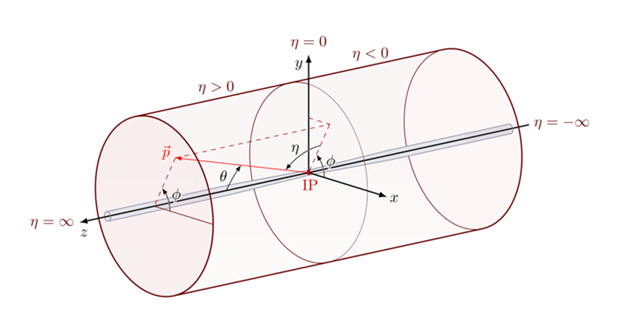
\includegraphics[width=12.5cm,height=6cm]{templates/CMS_coordinates.png}
    \caption{In the LHC, the beam direction is assumed to be in the $z$ axis, and the $x-y$ plane is perpendicular to the beam. $\theta$ is the angle between the particle momentum diirection and the $z$ direction. A particle with energy $E$ and momentum along the beam direction $p_z$ has rapidity $y \equiv \frac{1}{2} \ln \frac{E+p_{x}}{E-p_{x}}$ and pseudorapidity $\eta \equiv-\ln \tan \theta / 2$. Massless particles have $y=\eta$, and differences in rapidity are invariant under longitudinal (along the beam direction) boosts.}
    \label{CMS_coordinates}
\end{figure}
The most efficient and widely-used clustering algorithm is the anti-kt algorithm, usually implemented in the FastJet package.


After jets have been reconstructed, studying them can offer treasure trove of information about fundamental physics. One of the best best studied things in the LHC related to jets is the inclusive jet spectrum, which is related to the momentum transfer $2 \rightarrow 2$ scttering of partons inside the proton. In this process, the energy of a the jet is closely related to that of the hard scattering of partons inside the protons, therefore the inclusive jet spectrum quantifies the distributions of partons inside the proton.




Measurements of the inclusive jet and dijet cross sections are classical particle physics measurements and are benchmarks of the standard model at particle colliders. Such measurements have been measuren in $e^+ e^-, ep, pp,$ and $p \bar{p}$ colliders. They have been used to test the predictions of perturbative QCD, have given precise measurements of the strong coupling constant $\alpha_S$, have been used to obtain information about the structure of the photon and neutron by constraining parton distribution functions (PDFs) of theproton (as well as differentiate between PDF sets), and  have been used to look for possible deviations from the standard model.  








\section{What is a cross section and what are PDFs?}
The total scattering cross section is computed by convoluting the parton distibution function for each incoming parton from each proton with the corresponding partonic level cross section.

Hence, in the language of QCD, the short-distance (high energy) part of the process can be computed from perturbation theory, and long-distance (low energy) part of the process is driven by the non-perturbative nature of QCD at low-energy scales. Collinear factorization theorem allows us to separate the perturbative (calculable) hard part of the process from the non-pertubative one, which can be described in terms of parton distribution (or fragmentation) functions. The total cross section of inelastic proton-proton scattering to produce a final state $n$ can be calculated with the formula
\begin{equation}
    \sigma = \sum_{a, b} \underbrace{\int_{0}^{1} d x_{a} d x_{b} f_{a/A}\left(x_{a}, \mu_{F}\right) f_{b/B}\left(x_{b}, \mu_{F}\right)}_{\text{long-distance, non-perturbative PDF part}} \times \underbrace{\int d \Phi_{n}  \frac{1}{2 \hat{s}}\left|\mathcal{M}_{a b \rightarrow n}\right|^{2}\left(\Phi_{n} ; \mu_{F}, \mu_{R}\right)}_{\text{short-distance "hard" perturbative part}}
    \label{QCD_master}
\end{equation}
Where $f_{a/A}(x, \mu)$ denotes the parton distribution functions, which depend on the momentum fractin $x$ of a parton $a$ with respect to its parent hadron $A$, and on an arbitrary energy scale called the factorization scale $\mu_F$. $d \Phi_{n}$ is the differential phase space element over $n$ final-state particles,
\begin{equation}
    d \Phi_{n}=\prod_{i=1}^{n} \frac{d^{3} p_{i}}{(2 \pi)^{3} 2 E_{i}}(2 \pi)^{4} \delta^{(4)}\left(p_{a}+p_{b}-\sum_{i=1}^{n} p_{i}\right)
\end{equation}
Where $p_a$ and $p_b$ are the initial state momenta. 
The convolution of the squared matrix element $\left|\mathcal{M}_{a b \rightarrow n}\right|^{2}$ 
, averaged over initial-state spin and colour degrees of freedom, with the
Lorentz-invariant phase space Φn and multiplied by the flux factor $ 1/(2ˆs) = 1/(2xaxbs)$
results in the calculation of the parton-level cross section $\hat{\sigma}_{ab→n}$. 

Hence we can intuitively say that the differential cross section in transverse momenta of the observed jet can be factorized in the following form \footnote{sometimes this is called the "master formula"}
\begin{equation}
\frac{d \sigma_{jet}}{d \mathcal{O}} \sim\\
\sum_{a, b} \int d x_{a} f_{a / A}\left(x_{A}, \mu\right) \int d x_{b} f_{b / B}\left(x_{B}, \mu\right) \frac{d \sigma_{partons}}{\mathcal{O}}
\label{master}
\end{equation}
Where $\sigma_{partons}=\int d \Phi_{n}  \frac{1}{2 \hat{s}}\left|\mathcal{M}_{a b \rightarrow n}\right|^{2}\left(\Phi_{n} ; \mu_{F}, \mu_{R}\right)$ can be seen from \ref{QCD_master}, and $ \mathcal{O}$ is any jet observable for example the jet $p_T$ or the rapidity $|y|$. The equation \ref{master} illustrates the principle of \emph{factorization}  i.e. that short distance and long distance processes are separable such that they can be convoluted in this manner, so that the "hard part" $\sigma_{partons}$ and "normalizations" from the PDFs are on diffrent scales.   Factorization also posits that the PDFs are universal, i.e. process-independent. 


The parton level cross sections $d \sigma_{partons}$ has an expansion in powers of $\alpha_S$
\begin{equation}
    \frac{d \sigma_{partons}}{d P_{T}} \sim \sum_{N}\left(\frac{\alpha_{s}(\mu)}{\pi}\right)^{N} H_{N}\left(x_{A}, x_{B}, P_{T} ; a, b ; \mu\right)
    \label{patron_x}
\end{equation}
Where the coefficients $H_N$ are calculable in perturbative QCD. Equation \ref{parton_x} demonstrates the principle of \emph{Asymptotic Freedom}, i.e. hard scattering is weak at short distances, and hence perturbatively calculable. At next-to-leading-order and beyond, however, the calculation will involve divergences that must be removed, and the dependence on the scale $\mu$ will appear in their place. 

% Inclusive jet cross section measurements are typically defined by the anti-$k_T$ algorithm implemented in the FASTJET package. Such an algorithm is infrared-safe and boost-invariant along the z-axis. The algorithm has proven to be the most effective in keeping the background induced from pileup (i.e. from other interactions) under contril by keeping the jets circular in the $(y, \phi)$ plane with a radius radious roughly equal to the jet size parameter $R$.















\section{Short-term and long-term plan for my thesis}
As Run 3 will start later this year, the timing of my dissertation seems apt to analyze Run 1 and
2 data, as well as be one of the first to analyze Run 3 data. Although I have worked and still
work on many different projects in ML, PDFs, HGCAL, database, prefiring, my dissertation
will in a big picture view be composed of two parts: a short-term plan, which I define as my plan up to the next year, and a long-term plan, which is defined as my plan until I graduate, estimated to be 2 or 3 years. 

For my short term plan, I am going to be a part of a team at DESY that will use the full Run 2 dataset to measure the inclusive jet cross section. I plan to go to DESY this summer to work on this project, and our team plans to publish a paper on this measuremtn next year of which I will be one of the main co-authors.

For my long term plan, which will take the bulk of the writing that is to follow, I plan to do my own inclusive jet cross section measurement using the preliminary Run 3 data, but I will be using a novel observable for which there is only a single observable per event. This is done so that we can avoid cross problematic correlations between the different channels/bins. Having measured this cross section over the full $p_T$ range, we will use that to do a EFT fit. The novelty in our EFT fit is that this time we will do a true global fit, without making any assumptions about the EFT coeffiecients. This means that we will fit all the EFT (Wilson) coefficients simultaneously resulting in a full-scale modelling of the probability distributions of the Wilson coefficients. This would give the best chance of saying something about dimension-6 operators that might set bounds on new physics, as well as searching for contact interactions. 
\chapter{ My Previous Projects, and How They are Relevant and important}














\section{My previous projects}
This measurement requires many areas of expertise and skill, as it is one of the most difficult and ambitious measurements in modern particle physics. In preparation for this measurement, I have been building my skill sets and expertise in relevant particle physics research areas, here are a few research projects that I've worked on and how they are relevant in my preparation for this measurement.

\section{L1 Prefiring}
 As a member of the JETMET POG, I have worked on the L1 Prefiring problem for data collected in 2017 and 2018, and has made contributions and discoveries that has affected the entire CMS experiment. A brief summary of this issue is the following: from the end of 2016, certain jets and photons in the forward rejoin ($2<|\eta| <3$) were wrongly associated by the L1 trigger to be belonging to the previous bunch crossing, resulting in a loss of these events. This effect cannot be accounted for in MC, therefore a correction to MC must be applied to compensate for this loss of efficiency. A centrally produced map for the UL 2017 dataset was produced by me to account for this inefficiency. The probability map is in the $(p_T, \eta)$ plane of the jets or photons, and the probability of prefiring can be applied to MC jets/photons as weights to account for this inefficiency. Figure \ref{UL_2017} shows an example of the maps that I produced \footnote{These maps can be used for MC correction on CERN website [] }, but the interested reader should read my contributions to the JETMET POG presenting these results \cite{UL2017}. Working on this issue has given me the necessary tools and expertise and experience on how triggering is done in CMS, analyzing the behaviors of the various detectors in detail, as well as contributing to the experiment in a significant way.

\begin{figure}[h]%
    \centering
    \subfloat[\centering]{{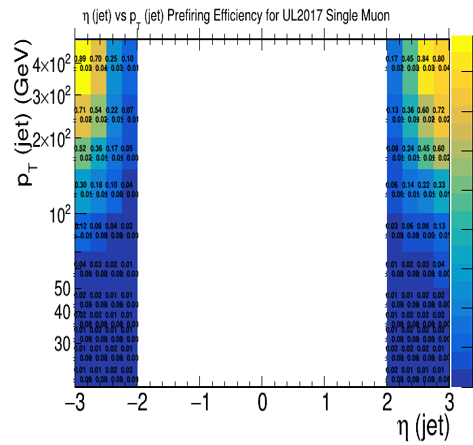
\includegraphics[width=7.05cm,height=6cm]{templates/images/UL17Pref_jetmap.png} }}%
    \qquad
    \subfloat[\centering]{{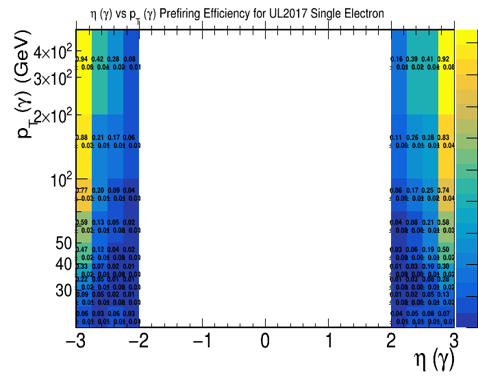
\includegraphics[width=7.05cm,height=6cm]{templates/images/UL17Pref_photonmap.png} }}%
    \caption{UL 2017 Prefiring Maps produced by Myself. The interested reader should also read my JETMET Contribution on this at \cite{UL2017}}%
    \label{UL_2017}%
\end{figure}




Recently, I performed this study again but this time for UL 2018 dataset. Myself and everyone else involved in these studies expected that we would see very small probabilities of prefiring for the UL 2018 data, since this problem was assumed to have been fixed. See for example \cite{Nick_Thomas} which describes how it was fixed. Indeed, my study concluded that this problem was fixed in the L1 trigger as the probabilities of prefired jets and photons were very low, as shown in figure. 
% UL 2018 2D MAPS
\begin{figure}[h]%
    \centering
    \subfloat[\centering]{{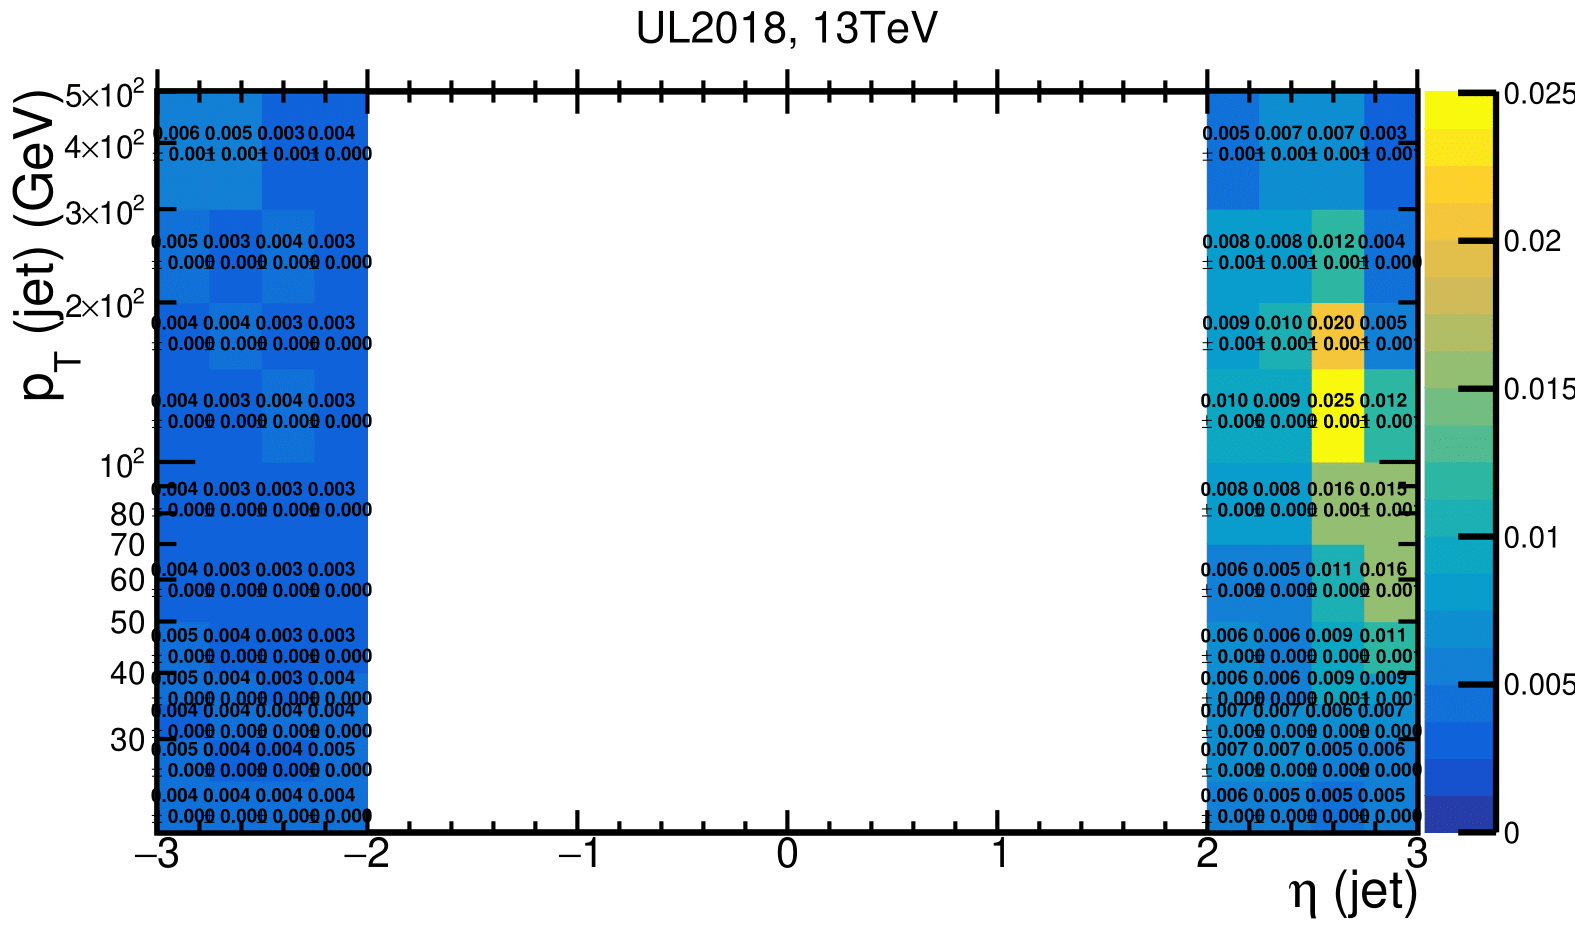
\includegraphics[width=4.5cm,height=5cm]{templates/images/JETptvseta_2D_UL2018-1.png} }}%
    \qquad
    \subfloat[\centering]{{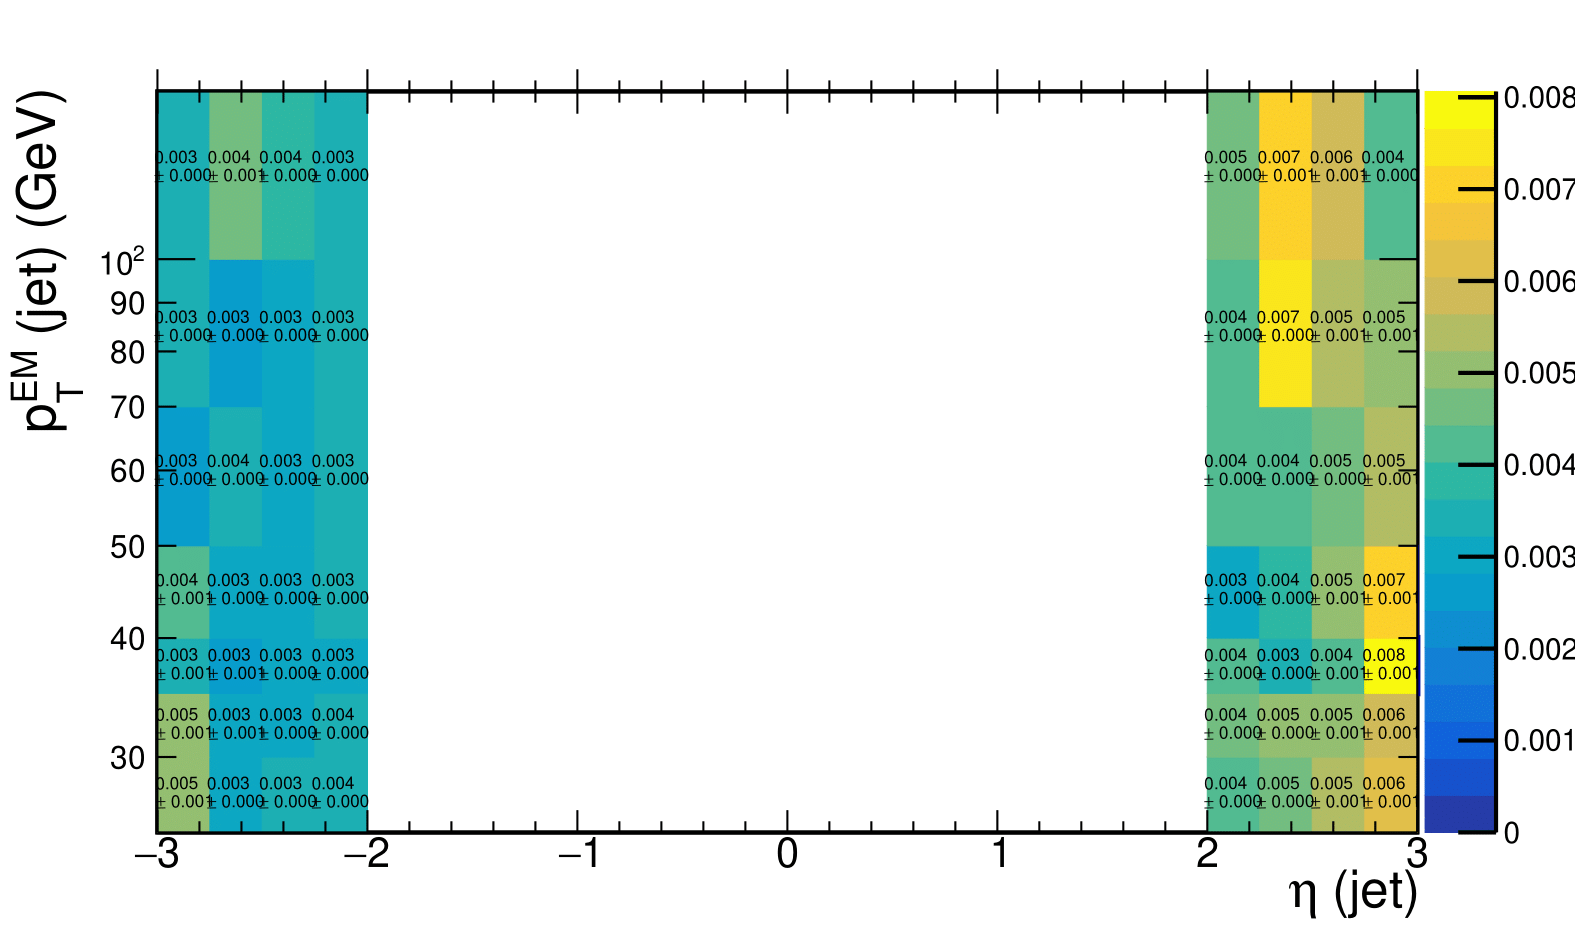
\includegraphics[width=4.5cm,height=5cm]{templates/images/JETEMptvseta_2D_UL2018-1.png} }}%
    \subfloat[\centering]{{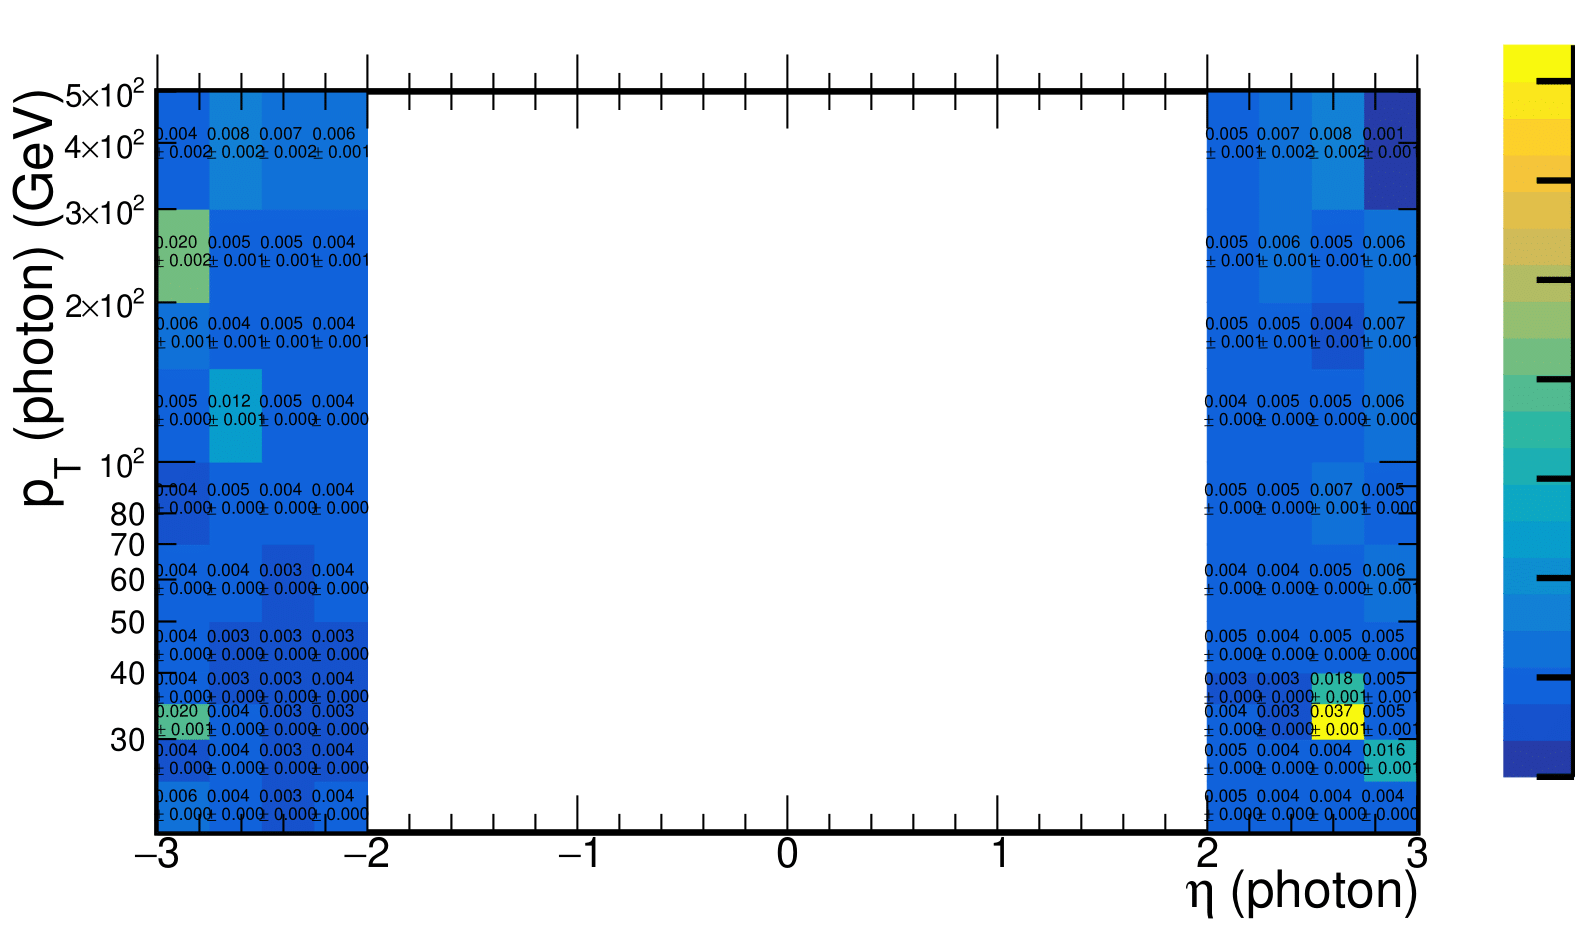
\includegraphics[width=4.5cm,height=5cm]{templates/images/PHOTONptvseta_2D_UL2018-1.png} }}%
    \caption{UL 2018 Prefiring Maps produced by Myself. The interested reader should also read my L1 DPG Contribution on this at \cite{UL2018}}%
    \label{UL_2018}%
\end{figure}

My studies on prefiring during 2018 showed two things that were unexpected. First, although the probabilities of prefiring were low overall, there was clear assymetry in prefiring probabilities for the $\eta>0$ region compared to the $\eta<0$ region (previously it was completely symmetric in $\eta$ previously, as sen in figure \ref{UL_2017}). This can be seen in figure \ref{UL_2018_RunA}. The other surprising thing was that the residual evident prefiring was coming from Run A, with a clear $\eta/ \phi$ structure, as seen in figure \ref{UL_2018_RunA}. Furthermore, I found that these effects were coming from two runs numbers in Run A where the L1 trigger misbehaved. My analysis was later fully confirmed by L1 DPG (see \cite{L1DPG}) by a different method, and as a result we removed these bad runs from the Golden JSON for 2018, affecting the entire CMS experiment.

%UL 2018 Run A
\begin{figure}[h]%
    \centering
    \subfloat[\centering Ratio efficiencies jets]{{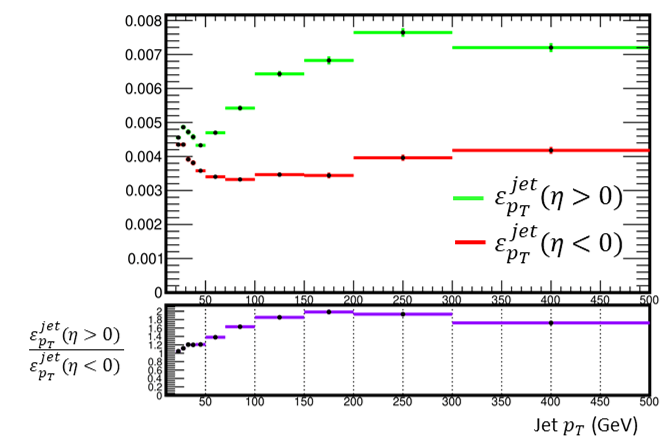
\includegraphics[width=5cm,height=5cm]{templates/images/Ratio_of_efficiencies_JETPT.png} }}%
    \qquad
    \subfloat[\centering Ratio of efficiences photon]{{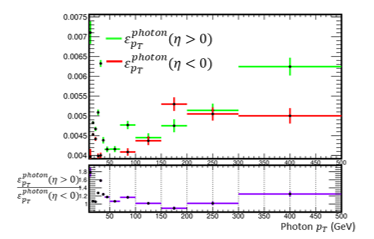
\includegraphics[width=5cm,height=5cm]{templates/images/Ratio_of_efficiencies_PHOTONPT.png} }}%
    \subfloat[\centering 1D hists]{{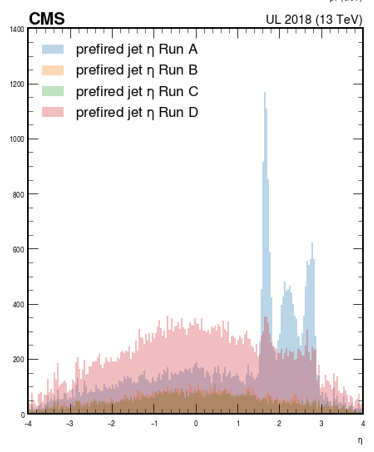
\includegraphics[width=5cm,height=5cm]{templates/images/1DHISTS_UL2018.png} }}%
    \subfloat[\centering Run A eta vs phi]{{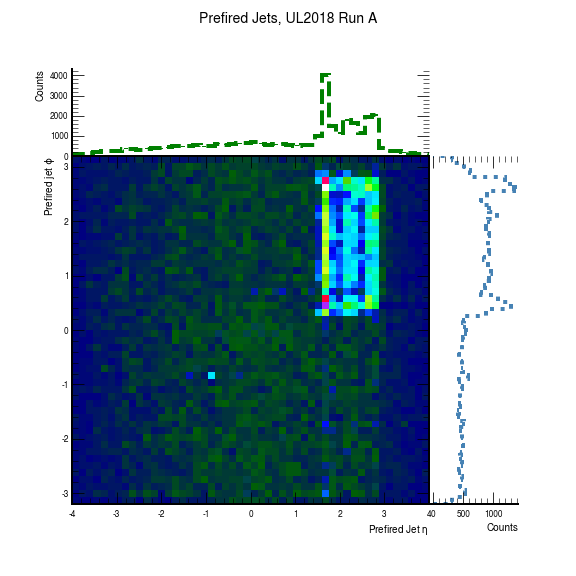
\includegraphics[width=5cm,height=5cm]{templates/images/Jet_phi_vs_eta_runA_PREFIRED.png} }}%
    \caption{UL 2018 Prefiring Maps produced by Myself. The interested reader should also read my L1 DPG Contribution on this at \cite{UL2018}}%
    \label{UL_2018_RunA}%
\end{figure}




As discussed in Chapter 1 (sec on the uncertainties included), there are many uncertainties and inefficiencies that enter the jet cross section measurement, and this is one of the inefficiencies that enter the calculation which has to be accounted for. Since I will be using Run 2 Data, correcting for this effect for my short-term plan will be crucial. 


\section{PDFs and xFitter}

As shown in Ch.1 sec on PDFs, PDF are paramount in jet cross section measurement and in any cross section measurement. Since there are many groups that routinely publish different PDF sets, a big problem in HEP is the proper characterization of these different PDFs and the quantification of their uncertainties and the uncertainties of the parameters that are included in different PDF sets, which was the aim of my studies in PDFs, where I used the PDF fitting software xFitter.

As discussed below, the reported PDF uncertainties and confidence intervals make some assumptions regarding the parameterization of the PDFs, which may not be statistically justified. A popular method for estimating the PDF errors is by constructing confidence intervals on the parameters using $-2 \log L$: suppose that the likelihood for $\theta$ is multivariate normal, the likelihood function of a single observation is of the form 
\begin{equation}
\begin{aligned}
    L(\boldsymbol{\theta} ; x)&=\frac{1}{\sqrt{(2 \pi)^{D}|\boldsymbol{\Sigma}|}} \exp \left\{-\frac{1}{2}[x-g(\boldsymbol{\theta})]^{T} \boldsymbol{\Sigma}^{-1}[\boldsymbol{x}-\mathrm{g}(\boldsymbol{\theta})]\right\} \\
    &= \frac{1}{\sqrt{(2 \pi)^{D}|\boldsymbol{\Sigma}|}} \exp \left\{-\frac{1}{2}\chi^2\right\}
\end{aligned}
\end{equation}
Taking the log and dropping the constant in the beginning (since the constant is independent of $\theta$), we have
\begin{equation}
\begin{aligned}
    \log L(\boldsymbol{\theta} ; \boldsymbol{x})&=-\frac{1}{2}[\boldsymbol{x}-\mathrm{g}(\boldsymbol{\theta})]^{\mathrm{T}} \boldsymbol{\Sigma}^{-1}[\boldsymbol{x}-\mathrm{g}(\boldsymbol{\theta})] \\
    &= - \frac{1}{2} \chi^2
\end{aligned}
\end{equation}

Thus, $-2 \log L$ is precisely the $\chi^2$ expression in the leaset squares method.
A popular method for estimating the errors in the maximum likelihood method is to look for parameters $\mathbf{\theta_{\pm}}$ for which
\begin{equation}
    -2 \Delta \log L \equiv-2\left[\log L\left(\boldsymbol{\theta}_{\pm} ; \boldsymbol{x}\right)-\log L(\hat{\boldsymbol{\theta}} ; x)\right]=1
\end{equation}
This method yields 68 \% confidence intervals on the individual parameters. These shifts in the parameters $\boldsymbol{\theta_{\pm}}$ can be attained with the maximum likelihood methodology. In other words, finding the points where $\Delta \chi^2=1$ corresponds to the method of finding the 68 \% confidence interval $( \hat{\theta} - \theta_+, \hat{\theta} + \theta_+ )$.

This method is widely used by all PDFs, but it is critical to remember that this assumes the normal sampling of $x$. If the sampling is not normal, then the probability content will be different, and must be determined for the correct sampling distribution. Since this method is used by xFitter and most other PDF fitting tools, we aim to study this assumption, whether it is true that the parameters that we aim to study are normally distributed. 

Our study aims at studying to what extent the PDF parameter marginalized densities (distributions) are normal (which is what PDF groups imply as discussed above), and whether we can retreive the actual parameter likelihoods, which might not be Gaussian, by a reweighting technique. We reweight the parameter points $\theta_i$ by the weight $w_i = \frac{L(\theta_i)}{\pi (\theta_i)}$ where $L(\theta_i)$ is the true likelihood for parameter $\theta$ at point $i$ and $\pi(\theta_i)$ is a prior or approximate likelihood of our choice, which assume $\Delta \chi^2 =1$. For example we could take it to be a multivariate Gaussian $\pi(\theta_i) = \mathcal{N} (\mu = \hat{\theta_i}, \Sigma = \hat{\Sigma})$, where $\hat{\theta_i}$ and $\hat{\Sigma}$ are the best-fit PDF values and their covariance matrix that are returned by xFitter, respectively. Our method shows promise for working in the limit of increasing datasets included in the PDF fit, due to the descrepancies between the different experiments which would affect the noramlity of the parameter distributions. For more details, please visit my Github repository, where all the code is available[], and to my invited talk at the 2022 xFitter Workshop \cite{xFitterWorkshop}.











%%%%%%%%%%%%%%%%%%%%%%%%%%%%%%%%%%%%%%%%%%%%%%%%%%%%%%%%%%%%%%%%%%%%%%%%%%%%%%%%%
\section{Quark/Gluon Jet Discrimination with ML}
The identification the origin of jets; whether they are quark or gluon jets, is an extremely important experimental test in uncovering the fundamental physics that occurs in a given event. One of the areas where quark-gluon jet identification is important is in understanding the properties of the Higgs. For example, if one wants to measure the Higgs boson coupling to gauge bosons, one would need to look at the weak-boson-fusion process $qq \rightarrow H qq$ (which makes quark jets) and not the more frequent gluon-fusion process $gg \rightarrow Hgg$ (which generates a gluon jet). In this project I used CMS Open Data to build machine learning classification models to classify between quark or gluon initiated jets. Using Baye's Theorem, $p(y \mid x)=\frac{p(x \mid y) p(y)}{p(x)}$ we therefore have the probability of observing a gluon jet given data $x$ as $p(\text{ gluon } |x) =\frac{p(x \mid \text { gluon }) p(\text { gluon })}{p(x \mid \text { gluon }) p(\text { gluon })+p(x \mid q u a r k) p(\text { quark })} $ which is the outcome of our ML classifier. An ensemble of all the state-of-the art classifiers that are available in common ML packages was studied in application to this problem, and the ML hyperparameters were all tuned to their optimal values using random grid search. The best performing classifier, as indicated by the ROC curves in figure \ref{ROC_QG}. Perhaps more interestingly, I found that the jet observable that resulted in the greatest discrimination power between quark and gluon jets was the jetQCI variable, which was constructed on the basis that gluon jets are wider than quark jets, as seen in figure \ref{QGI}. see \cite{QGI} for more details.

\begin{figure}[h]%
    \centering
    \subfloat[\centering ROC Curves for classifiers whose hyperparameters were tuned with grid search]{{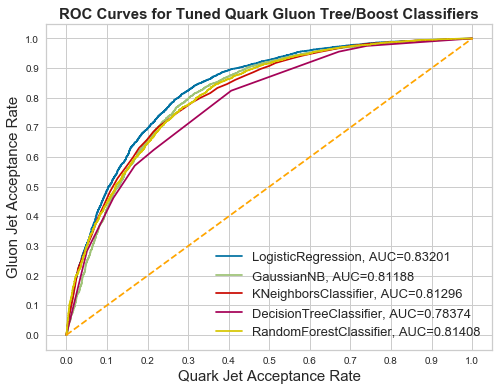
\includegraphics[width=7cm,height=5cm]{templates/ROC_TUNED.png} }}%
    \qquad
    \subfloat[\centering The jet observables that yield the greatest discrimination power between quark and gluon jets. The winner is the jetQGI variable, which is denoted as $\sigma$ in \cite{QGI}]{{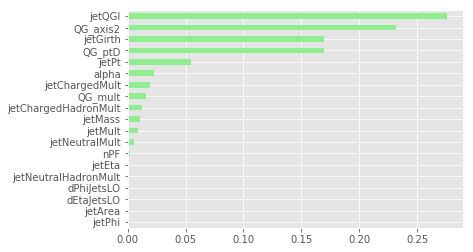
\includegraphics[width=7cm,height=5cm]{templates/images/feature_importance.png} }}%
    \caption{UL 2017 Prefiring Maps produced by Myself. The interested reader should also read my JETMET Contribution on this at \cite{UL2017}}%
    \label{QGI}%
\end{figure}
This study was later extended to consider a more realistic model for quarks and gluons. Recall that the objective of any classifier is to approximate the function 
\begin{equation}
    \begin{aligned}
f^{*} &=P(t=1 \mid x) \\
&=\frac{p(x \mid s) \pi(s)}{p(x \mid s) \pi(s)+p(x \mid b) \pi(b)}
\end{aligned}
\end{equation}

In other words, the function $f^∗$ (or classifier) approximates the discriminant
\begin{equation}
    D(x)=\frac{s(x)}{s(x)+b(x)}
\end{equation}

However, this discriminant assumes ideal and \emph{pure} probability densities $g(x)$ and $q(x)$. The actual densities of the samples have quark densities that include mixtures of the other quark flavor, and since we are only considering binary classification of quark and gluon jets, the actual densities are
\begin{equation}
\begin{aligned}
&G(x)=\left(1-\epsilon_{q}\right) g(x)+\epsilon_{q} q(x) \\
&Q(x)=\left(1-\epsilon_{g}\right) q(x)+\epsilon_{g} g(x)
\end{aligned}
\end{equation}
Where the fractions $\epsilon_g$ and $\epsilon_q$ are mixture fractions corresponding to the two jet flavors. Hence we can define the actual, or \emph{contaminated discriminant} $D'(x)$, which is what we are actually approximating by the classifiers, which includes the mixture fractions
\begin{equation}
    D^{\prime}(x)=\frac{G(x)}{G(x)+Q(x)}
\end{equation}
Which, after subsitituting $G$ and $Q(x)$ and simplifying
\begin{equation}
    D^{\prime}(x)=\frac{\epsilon_{q} q(x)_{g}(x)\left(1-\epsilon_{q}\right)}{\epsilon_{g} g(x)-\epsilon_{g}+\epsilon_{q} q(x)+g(x)\left(1-\epsilon_{q}\right)+1}
\end{equation}
Now, what is interesting is that $D'(x)$ can be represented in terms of $D(x)$
\begin{equation}
    D^{\prime}=D \frac{(g+q)(e q q+g(1-e q))}{g(e g g-e g+e q q+g(1-e q)+1)}
\end{equation}
This means that the realistic contaminated discriminant is a function of $D$ only since $\epsilon_q$ and $\epsilon_g$ are constants. Furthermore, the fact that $D'$ is one-to-one with $D$ means that their discrimination power is the same.  This means that the optimal discriminant $D$ can be computed from
$D'$, where the contamination fractions are given in $D'$
, and by studying the relationship between $D$ and $D'$ over the range of $\epsilon_q$ and $\epsilon_g$ one could identify where
the relationship between them is monotonic.

This project was one of my first applications of machine learning to a particle physics problem and it yielded some interesting results, and a possibility of arriving at an optimal quark-gluon classifier by the contaminated classifier technique described above. It also taught me the power of machine learning in jet studies and how one has freedom to construct jet observables, which becomes all the more powerful if it is informed by intuition and machine learning. Constructing similar observable will be very important for my thesis plan.




%%%%%%%%%%%%%%%%%%%%%%%%%%%%%%%%%%%%%%%%%%%%%%%%%%%%%%%%%%%%








\section{Observable with high $p_T$ jets and the Response Matrix}
\label{jet_order_response}

My goal first in this project was to explore and quantify to what extent the $p_T$ of highest-$p_T$ jet in an event can be used as an observable. My second goal was to study how we can construct the "response matrix" which is a mapping from "true" or theoretical (or generated - gen for short) values to the measured (or reconstructed - rec for short) values, in the context of the jet $p_T$. In CMS analyses, this mapping is done via
\begin{equation}
    \mathbb{P}\left(p_{T}^{\text {rec }} \mid p_{T}^{g e n}\right)=   \mathbb{P}\left(p_{T}^{\text {gen }} \mid \mathrm{SF} \right)
    \times\left(1+\mathrm{SF} \times \Delta_{\mathrm{MC}} R_{G}\right)
\end{equation}
Where $\Delta_{\mathrm{MC}}    =\frac{p_{T}^{\mathrm{rec}}-p_{T}^{\mathrm{gen}}}{p_{T}^{\mathrm{gen}}}$ is the "resolution", $R_G$ is a random number sampled from a standard normal distribution \footnote{meaning $\mu=0, \sigma=1$} and \mathrm{SF} are smearing factors which are extracted from the measurement of the resolution of the data, and are provided centrally at CMS by JetMET. We argue that this mapping makes unproven assumptions (such as the normality of the smearing) and it requires exact knowledge of the smearing factors, which are nuissance parameters, making it very inconvenient.




In our study, we aim to "fold" the gen jet ($p_T$) spectrum by the respense function  $\mathbb{R}\left(p_{T}^{r e c} \mid p_{T}^{\text {gen }}\right)$ by calculating the integral 
\begin{equation}
    \mathbb{P}\left(p_{T}^{\text {rec }} \mid p_{T}^{g e n}\right)=\int \mathbb{R}\left(p_{T}^{r e c} \mid p_{T}^{g e n}\right) f\left(p_{T}\right) d p_{T}
\end{equation}
Where $f(p_T)$ is the true spectrum of the leading jet. The Data is consistent of pythia 8 (CUEITP8M1) MC samples with $2 \rightarrow 2$ parton-parton interactions included
in the matrix element (ME): these will be referred to as ”gen” or generator (truth) samples. \footnote{Multiparton interaction, initial state
radiation, FSR and hadronization were also simulated in the MC samples}
In order to study the detector-related effects, the CMS detector
response is also simulated using the GEANT4 package. These will be referred to as the ”rec” samples. The distributions for the jet kinematic variables $\left(p_{T}, \eta, \phi\right)$ were constructed for $\approx$ 9 Million events, each having a varying number of jets per event. Before we are able to to further analyze these samples and assess the detector response, we must have a one-to-one mapping of each gen jet to its corresponding rec jet. This is done via matching in $(\eta, \phi)$ space, where the distance between a gen (1) jet and a rec (2) jet was chosen nto be within a cone of radius $\Delta R_{12}=\sqrt{\Delta y_{12}^{2}+\Delta \phi_{12}^{2}} < 0.25$.

In order to study the kinematic variables of the reco and gen jets, we can
use the $p_T$ ordering of the jets as a means to quantify whether the $p_T$ of the highest jet can be used as an observable. One way to tell whether it can be used as an observable is to calculated the probability of flipping of the order of the gen jets compared to rec jets, $\mathbb{P}_{f l i p}(g e n, r e c)$: what is the probability that the order of the $p_T$ of the rec jets is flipped when ordered according to the $p_T$ order of the gen jets?

Hence, if we show that there is a nonzero flipping probability for the first jet, i.e. there is a probability that the leading gen jet corresponds to a non-leading reco jet, the response
function has to be modified in order to be compared to the provided
theoretical distribution by multiplying the integral by a flipping probability
\begin{equation}
    \mathbb{P}\left(p_{T}^{r e c} \mid p_{T}^{g e n}\right)=\int \mathbb{R}\left(p_{T}^{r e c} \mid p_{T}^{\text {gen }}\right) f\left(p_{T}\right) \mathbb{P}_{f l i p}\left(p_{T}^{r e c}, p_{T}^{g e n}\right) d p_{T}
\end{equation}

For our task, we want to find the conditional distribution $\mathbb{P}\left(p_{T}^{r e c} \mid p_{T}^{g e n}\right)$. This can be done via a Machine Learning and a "likelihood ratio trick" (see for example [arXiv:1805.12244v4] which also uses this in a HEP application). Given a classification model, which tries to find the mapping $p_T^{rec} = f(p_T^{gen})$, which can be estimated as $\hat{f}$

\begin{equation}
f(p_T^{rec}) \approx \hat{f}(p_T^{gen})=\arg _{\hat{f}} \min \int L(p_T^{rec}, \hat{f}) \ p(p_T^{rec} | p_T^{gen}) d y
\end{equation}
Where $ L(p_T^{rec}, \hat{f})$ is a (binary classification) loss function.

Hence our task is to approximate the optimal classifier, which, given training data $x$ learns

\begin{equation}
d(x)=\frac{\mathbb{P}\left(x | p_T^{rec}\right)}{\mathbb{P}\left(x | p_T^{gen}\right)+\mathbb{P}\left(x | p_T^{rec}\right)}=\frac{f(x)}{1+f(x)}
\end{equation}


Where $f$ is the classifier decision function, Which is 1-to-1 with the likelihood ratio,
\begin{equation}
\hat{r} (x| p_T^{gen}, p_T^{rec})=\frac{\mathbb{P}\left(x | p_T^{rec}\right)}{\mathbb{P}\left(x | p_T^{gen}\right)}
\end{equation}
Which can be written as 

\begin{equation}
\hat{r} (x| p_T^{gen}, p_T^{rec})=\frac{\mathbb{P}\left(x | p_T^{rec}\right) \ \mathbb{P}(p_T^{rec})}{\mathbb{P}\left(x | p_T^{gen}\right) \ \ \mathbb{P}(p_T^{rec})} =\frac{d(x)}{1-d(x)}
\end{equation}
Our posterior density could finally be calculated as
\begin{equation}
    \mathbb{P}\left(p_{T}^{r e c} \mid p_{T}^{g e n}\right)=\frac{d}{1-d} \times f\left(p_{T}^{r e c}\right)
    \label{ratio_trick_posterior}
\end{equation}

In building our probabilistic machine learning model, we have the target class corresponding to the true $p_T^{gen}$ and the normalized distribution of the rec jets $Z= \frac{p_T^{rec}}{p_T^{gen}}$
\begin{equation}
    \left\{p_{T}^{\text {gen }}, Z=\frac{p_{T}^{r e c}}{p_{T}^{\text {gen }}}\right\}, \text { Target }=1
\end{equation}
And the other class corresponding to a distribution that is randomly sampled from $p_T^{gen}$ and a random sampling of the $Z$ distribution, $f(Z)$:
\begin{equation}
    \left\{f\left(p_{T}^{g e n}\right), f(Z)=f\left(\frac{p_{T}^{r e c}}{p_{T}^{g e n}}\right)\right\}, \text { Target }=0
\end{equation}
We pick $f(Z)$  to be randomly sampled from a Gaussian with mean $\mu=\frac{p_{T}^{r e c}}{p_{T}^{\text {gen }}}$ and standard deviation corresponding to the width of the $Z$ distribution, i.e.
\begin{equation}
f(Z)=\frac{1}{\sigma \sqrt{2 \pi}} e^{-\frac{1}{2}\left(\frac{p_T^{rec}-p_T^{gen}}{\sigma}\right)^{2}}
\end{equation}
Therefore the function $f(Z)$ can be regarded as a rough approximation of the distribution $Z$, and given this, $\frac{d}{1-d}$ fixes the approximation.

The posterior distribution from our model in equation \ref{ratio_trick_posterior} was compared to the simulated data which corresponds to the true CMS detector response. These "data" were simulated with Delphes by passing the truth distribution (which was generated with Pythia) to Delphes to reconstruct the jets given the detector response and smearing, using the CMS card. Results using this method is shown in figure

\begin{figure}[h]%
    \centering
    \subfloat[\centering]{{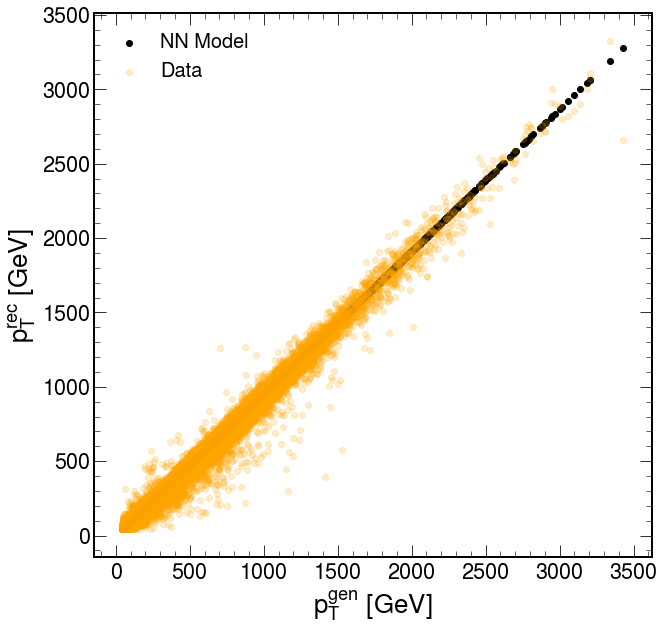
\includegraphics[width=4.5cm,height=5cm]{templates/NN_data_dist.png} }}%
    \qquad
    \subfloat[\centering]{{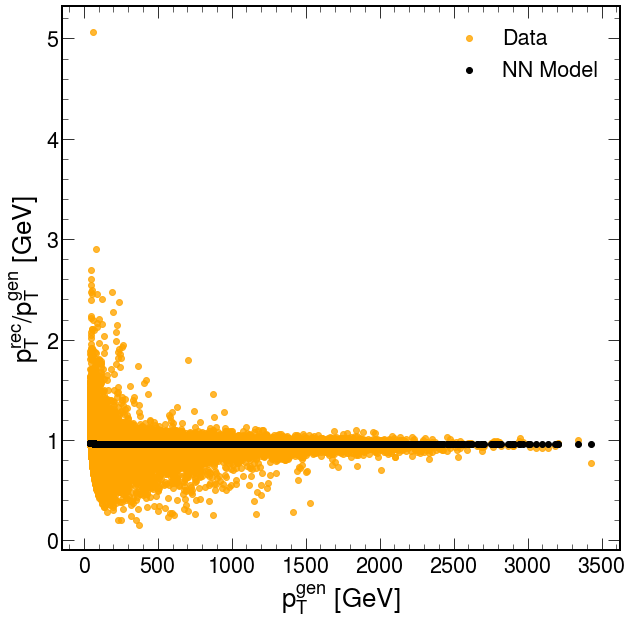
\includegraphics[width=4.5cm,height=5cm]{templates/re_div_gen_model_data.png} }}%
    \subfloat[\centering]{{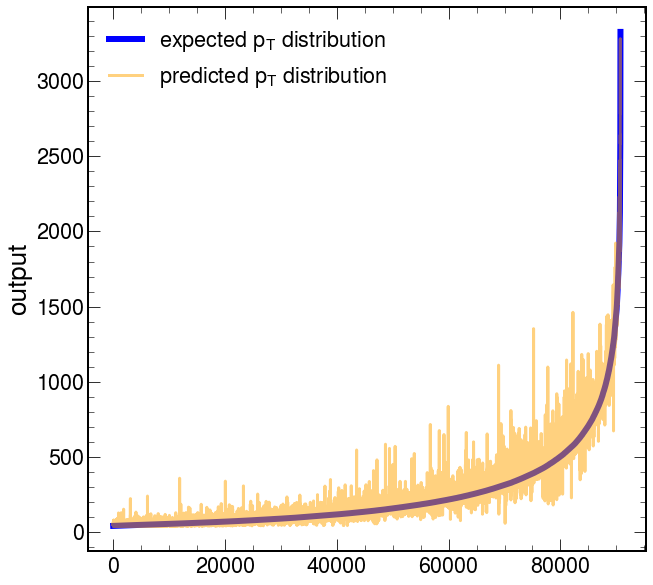
\includegraphics[width=4.5cm,height=5cm]{templates/expected_dist_pt.png} }}%
    \caption{(a): "Response matrix" for matched jets }%
    \label{ratio}%
\end{figure}





















\chapter{Doing Jet Cross section for Run 3, Doing EFT Fit and Searching for Contact Interactions}

\section{Doing the Jet Cross section for Run 3 and The Relevant Uncertainties}
As mentioned earlier, I plan to measure the inclusive jet differential cross section for the preliminary Run 3 data. The LHC will start collecting data again for Run 3 in early 2023. As a PhD student, I will be among the first to  analyze Run 3 data in the context of an inclusive jet spectrum. In what follows I shall give a brief overview of what is measuting this cross section means from an experimental point of view, as well as all the uncertainties that are involved, and the importance of observables in this measurement.


The inclusive jet cross section is $\sigma (pp \rightarrow \text{jet} + X)$, where $X$ signifies "anything". It is usually measured as a function of the jet transverse momentum, $p_T$,  and absolute rapidity $|y|$, hence a common measurement inclusive jet double-differential cross section is $\frac{d^2 \sigma}{dp_T dy}$.

Once my samples for the preliminary Run 3 have been obtained, jets are isolated, reconstructed and corrected, ensured to pass criteria, etc., The measured inclusive double differential jet cross section looks like
\begin{equation}
    \frac{\mathrm{d}^{2} \sigma}{\mathrm{d} p_{T} \mathrm{~d}|y|}=\frac{1}{\epsilon \mathcal{L}} \frac{N_{\text{jets}}}{\Delta p_{T} \Delta|y|}
\end{equation}
Where $\Delta p_T$ and $\Delta |y|$ are the corresponding bins widths. The rapidity intervals are chosen, for example $\Delta |y|=0.5$, $N$ is the number of jets in the corresponding $p_T$ bin, $\mathcal{L}$ is the effective integrated luminosity of the data sample taking into account the trigger prescales, $\epsilon$ is the product of all the jet selection and trigger efficiencies. Similarly the inclusive double-differential cross section for the dijet mass is
\begin{equation}
    \frac{d^{2} \sigma}{d M_{j j} d|y|}=\frac{1}{\epsilon \mathcal{L}} \frac{N_{\text{jets}}}{\Delta M_{j j} \Delta|y|}
\end{equation}
Where $M_{jj}$ is the dijet invariant mass.
%Previous measurements can be seen in figure.

Any source of error that affects the $p_T$, $M_{jj}$ or any other observable that might affect the studied jet cross section must be discussed as a source of uncertainty. The experimental uncertainties that come into this measurement are numerous and complex, and could constitute a PhD thesis on their own.(eg see the CMS JES paper). In summary, the experimental uncertainties come from imperfect measurement of jet energy and jet $p_T$, imprecise simulation of jet energy resolution, imprecise knowledge of integrated luminosity. These inefficiencies are taken to be factorized into multiple uncertainties that are important to discuss.


\section{The importance of Jet observables }
All cross section measurements in hadron colliders can be described by the "master formula", such as equation \ref{QCD_master} discussed earlier. We can write a simpler version describint a scattering process where we have beams $A$ and $B$ coming in and final states $1\ 2\ 3\ ... \ n$ coming out. If we want to compute the cross section for some observable $\sigma_{\text{obs}}$ a simplified master formula, assuming the beams are massless, is
\begin{equation}
    \sigma_{o b s}=\frac{1}{E_{C M}^{2}} \sum_{n=1}^{\infty} \int d \phi_{n}\left|\mathcal{M}_{A B \rightarrow 12 \ldots n}\right|^{2} f_{o b s}\left(\phi_{n}\right)
\end{equation}
where $E_{\text{CM}}$ is the center of mass energy, the sum is over all the final states, and the integral is over the lorentz-invariant $n$-body phase space $\phi_n$ (i.e. over everywhere these particles go). $\left|\mathcal{M}_{A B \rightarrow 12 \ldots n}\right|$ is the hard scattering amplitude, and $f_{o b s}\left(\phi_{n}\right)$ is what we choose as an observable, which depends on the phase space or kinematics of the outgoing particles. The problem for jets is that the final states we measure, $1\ 2\ 3\ .... \ n$, are hadrons, but the scattering amplitudes that we can calculate, $\mathcal{M}$ are in terms of quarks and gluons. Therefore we have to somehow bridge the divide between the types of calculations whose scattering amplitudes we can calculate perturbatively, and the types of measurements that we can take which are composed of hadronic final states. The key to bridging this gap is the choice of observables in an appropriate "factorizable" way.








\section{SMEFT Fit and Contact Interactions Search}
The Standard Model Effective Field Theory (SMEFT) is a consistent effective field theory generalization of the SM built out $\mathrm{SU}_{\mathrm{c}}(3) \times \mathrm{SU}_{\mathrm{L}}(2) \times \mathrm{U}_{\mathrm{Y}}(1)$ higher dimensional operators, composed of SM fields. The SMEFT is defined as 
\begin{equation}
    \mathcal{L}_{S M E F T}=\mathcal{L}_{S M}+\mathcal{L}^{(5)}+\mathcal{L}^{(6)}+\mathcal{L}^{(7)}+\ldots
\end{equation}
Where 
\begin{equation}
    \mathcal{L}^{(d)}=\sum_{i=1}^{n_{d}} \frac{C_{i}^{(d)}}{\Lambda^{d-4}} Q_{i}^{(d)} \quad \text { for } d>4
\end{equation}
Where $Q_{i}^{(d)}$ are the operators, which are suppressed by $d-4$ powers of the cutoff scale $\Lambda$ and the $C_{i}^{(d)}$ are the Wilson coefficients. See e.g. https://arxiv.org/pdf/1706.08945.pdf for a review.
% \begin{equation}
%     \mathcal{L}_{\text{contact interactions}} \in \mathcal{L}^{(6)} ? 
% \end{equation}
Why $d=6$ is the most interesting set of operators.

It is important to note that a  constraint that physial cross sections are semi-positive definite quantities, which can be accounted for in global SMEFT analyses. Consider, for example, the SMEFT Lagrangian
\begin{equation}
    \mathcal{L}=\mathcal{L}_{\mathrm{SM}}+\sum_{i=1}^{n_{\mathrm{op}}} \frac{c_{i}}{\Lambda^{2}} \mathcal{O}_{i}
\end{equation}
Where $\mathcal{O}_{i}$ are the dimension-6 operators and $c_i$ are the Wilson coefficients, which are assumed to be real (do they have to be?). Then any observable, such as the cross section, calculated using this Lagrangian can be written as the expansion
\begin{equation}
    \begin{aligned}
\sigma &= \underbrace{c_{0}^{2} \sigma_{00}}_{\text{SM contribution}} \\
&+\underbrace{c_{0} c_{1} \sigma_{01}+c_{1} c_{0} \sigma_{10}+c_{0} c_{2} \sigma_{02}+\ldots}_{\text{linear $\mathcal{O}\left(\Lambda^{-2}\right)$ EFT contributions}} \\
&+\underbrace{c_{1}^{2} \sigma_{11}+c_{1} c_{2} \sigma_{12}+c_{1} c_{3} \sigma_{13}+\ldots}_{\mathcal{O} (\Lambda^{-4}) \text{contributions}} \\
&=\boldsymbol{c}^{T} \cdot \boldsymbol{\Sigma} \cdot \boldsymbol{c}
\end{aligned}
\end{equation}

And since the physical cross section must be either positive or null, the matrix $\boldsymbol{\Sigma}$ must be semi-positive-definite. The Sylvester criterion requires the constraints coming from the $2\times 2$ minors as $\left(\Sigma_{i i} \Sigma_{j j}-\Sigma_{i j}^{2}\right) \geq 0, \quad i, j=0, \ldots n_{\mathrm{op}}$. Using this convention for the dimension-6 SMEFT, a genereic LHC cross section will be modified as
\begin{equation}
    \begin{aligned}
    \sigma_{\text{LHC}} &=\sigma_{\mathrm{SM}}+\sum_{i=1}^{n_{\mathrm{op}}} c_{i} \sigma_{i}^{\text{EFT}}+\sum_{i<j}^{n_{\mathrm{op}}} c_{i} c_{j} \sigma_{i j}^{\text{EFT}}
    \end{aligned}
\end{equation}


The quality of the global fit as well as the statistical model will be discussed in detail in the next chapter, but let us suppose that we are using a $\chi^2$ function as is typically used.
The quality of a global fit can be obtained by minimizing the log-likelihood, or the $\chi^2$ function, which compares the theoretical predictions to the experimental data by means of a covariance matrix. In this case is defined by 
\begin{equation}
    \chi^{2}(\boldsymbol{c}) \equiv \frac{1}{n_{\text {dat }}} \sum_{i, j=1}^{n_{\text {dat }}}\left(\sigma_{i}^{(\mathrm{th})}(\boldsymbol{c})-\sigma_{i}^{(\exp )}\right)\left(\operatorname{cov}^{-1}\right)_{i j}\left(\sigma_{j}^{(\mathrm{th})}(\boldsymbol{c})-\sigma_{j}^{(\exp )}\right)
    \label{chi2_EFT}
\end{equation}
Where $\sigma_{i}^{(\exp )}$ and $\sigma_{i}^{(t h)}(\boldsymbol{c})$ are the central experimental data and corresponding theoretical prediction, which depends on the Wildon coefficiencts $\boldsymbol{c}$, for the i-th cross section. Note that equation \ref{chi2_EFT} is precisely \emph{not} what we want to do! We are including it here since this is what is currently done in all such fits. See Chapter \ref{stats_likelihood} for a more on this.
A theoretical cross section depends on all the Wilson coefficients, and the exact dependence on each coefficient, say the EFT coefficient $c_j$ can be found by varying $c_j$ while setting the rest of the coefficients to zero, so that 
\begin{equation}
    \sigma_{m}^{(\mathrm{Th})}\left(c_{j}\right)=\sigma_{m}^{(\mathrm{SM})}+c_{j} \sigma_{m, j}^{(\mathrm{EFT})}+c_{j}^{2} \sigma_{m, j j}^{(\mathrm{EFT})}
\end{equation}
which results in a quartic polynomial form for the $\chi^2$, which can be expanded as $\chi^{2}\left(c_{j}\right)=\sum_{k=0}^{4} a_{k}\left(c_{j}\right)^{k}$ and minimized to obtain the best-fit value of the coefficient, $c_{0,j}$. See also [Combined SMEFT interpretation of Higgs, diboson,
and top quark data from the LHC]] for more details.
Note however, that equation \ref{ch2_EFT} assumes that the data are Gaussian distributed around the true SM values, which may or may not be a good approximation. This also assumes that the covariance matrix can be expressed as a sum of separate experimental and theoretical covariance matrices, and hence that the experimental and theoretical uncertainties are uncorrelated
\begin{equation}
    \operatorname{cov}_{i j}=\operatorname{cov}_{i j}^{(\exp )}+\operatorname{cov}_{i j}^{(\text {th })}
\end{equation}

Where the experimental covariance matrix is constructed from all sources of statistical and
systematic uncertainties that are made available by the experiments. EFT theorists therefore use only the full covariance matrix, without details of its individual components. This complicates EFT fit reinterpretations, because the covariance matrices have to be modifidied to include more data, additional uncertainties, etc. Furthermore, the provided covariance matrix is not necessarily positive-definite or it is ill-defined. In this case, the dataset is either discarded for the fit or its covariance matrix is regularized by some ad-hoc procedure. All these problems (there's more) would be avoided if one publishes the full statistical model together with the data, since one can then construct the exact likelihood function without the need of any ad-hoc approximations and exploit the complete information offered by CMS data.

\subsection{Search for Contact Interactions}

Quark compositeness models assume that quarks are composed of more fundamental particles with new strong interactions at a composite scale $\Lambda$, much greater than the quark masses. At energy much below $\Lambda$, quark contact interactions (CI) are induced by the underlying strong dynamics, and yield observable signals at hadron colliders. It is modeled that the contact interactions are induced by an effiective $d=6$ Lagrangian, given by
\begin{equation}
    \mathcal{L}_{CI}=\frac{1}{2 \Lambda^{2}}\left(c_{1} O_{1}+c_{2} O_{2}\right)
\end{equation}
Where here it is considered that the quark contact interactions are products of left-handed electroweak isoscalar quark currents which are assumed to be flavor-symmetric to avoid large flavor-changing neutral-current interactions, (arXiv:1101.4611v2) $c_1, c_2$ are the Wilson coefficients, and $O_1, O_2$ are the relevant four-fermion operators. 
\footnote{$O_{1}=\delta_{i j} \delta_{k l}\left(\sum_{c=1}^{3} \bar{q}_{L c i} \gamma_{\mu} q_{L c j} \sum_{d=1}^{3} \bar{q}_{L d k} \gamma^{\mu} q_{L d l}\right)$,  $O_{2}=\mathrm{T}_{i j}^{a} \mathrm{~T}_{k l}^{a}\left(\sum_{c=1}^{3} \bar{q}_{L c i} \gamma_{\mu} q_{L c j} \sum_{d=1}^{3} \bar{q}_{L d k} \gamma^{\mu} q_{L d l}\right)$ where $c,d$ are generation indices, $i, j, k, l, a$ are color indices, $T^a$ are the Gell-Mann matrices with the normalization $\operatorname{Tr}\left(\mathrm{T}^{a} \mathrm{~T}^{b}\right)=\delta^{a b} / 2$.}


In the SM, QCD predicts that jets are preferabbly produced in large rapidity bins, via small angle scattering in t-channel processes. Furthermore, it predicts that the $p_T$ or $M_{jj}$ spectrum falls off very fast at large values. On the other hand, jet production induced by contact interactions (such as $qq \rightarrow qq$) is expected to be much more isotropic and fall off slower with increasing values of $p_T$ or $M_{jj}$. CI models also predict that the region that is most sensitive to CI are low rapidity region. This is why it was shown that the inclusive jet $p_T$ and the dijet anglular distribution, show a great sensetivity to possible quark contact interactions induced by SMEFT (new physics) models. The dijet angular variable is $\chi_{\mathrm{dijet}}=\exp \left(2 y^{*}\right)$, where $y^{*}=\frac{1}{2}\left|y_{1}-y_{2}\right|$ where $\pm y^{*}$ are the rapidities of the two jets in the parton-parton c.m. frame.



The theoretical jet cross sections could be calculated using the CI scale $\Lambda$ and Wilson coefficients $c_i$, and this cross section, interestingly, could be decomposed into a cross section per each kinematic bin %(file:///D:/PROSPECTUS/RELEVANT_PAPERS/CIJET_GAO.pdf)
\begin{equation}
\begin{aligned}
    \sigma_{b i n}^{theor} &=\sum_{i=1}^{6}\left(\lambda_{i}\left(b_{i}+a_{i} r\right)\right) / \Lambda^{2} +\sum_{i=1}^{6}\left(\lambda_{i}^{2}\left(b_{i i}+a_{i i} r\right)\right) / \Lambda^{4} \\
    &+ \sum_{i=1,3,5}\left(\lambda_{i} \lambda_{i+1}\left(b_{i i+1}+a_{i i+1} r\right)\right) / \Lambda^{4}  +\sum_{i=1,2,5,6}\left(\lambda_{i} \lambda_{4}\left(b_{i 4}+a_{i 4} r\right)\right) / \Lambda^{4}
    \label{xsec_Gao}
\end{aligned}
\end{equation}
Where $c_{i}=4 \pi \lambda_{i}, r=\ln \left(\Lambda / \mu_{0}\right)$, and $\mu_0$ is an arbitrary reference scale chosen according to the kinematic range of the bin. 

% Having our theoretical cross section will be the one that is calculated with, say Gao's code, which is what is input into equation \ref{chi2_EFT}

Measure $\sigma^{exp}$ with a good observable in which there is only one instance per event $\rightarrow$ calculate  $\sigma^{theor}$ from $xsec_Gao$ using that observable $\rightarrow$ Fit $\sigma^{theor}$ and $\sigma^{exp}$ to set limits on Wilson coefficients $\rightarrow$ Are there CI's? (set limits on $\Lambda$).









\section{Defining My Own Observable}
With the intention of only having one observable per event to avoid cross-bin correlation, and informed by SMEFT.



\chapter{Statistical Model and Publishing the Likelihood}
\label{stats_likelihood}
Why publish the likelihood, etc.




\section{Statistical Model}
Supose that a set of $N_c$ independent channels for events are defined, in my case the channels could be distinct physics channels (processes leading to jets) or bins of a histogram. A certain number of events $n_i$ is found in channel $i$ and for every event $j$ in that channel one measure a vector of values $x_{ij}$. Suppose the $n_i$ counts can be modeled as independent and Poisson-distributted with mean counts $\nu_i (\mu, \theta)$ (typically $\nu_i (\mu=\sigma, \theta=\{ \mathcal{L}, \text{BR}, \varepsilon \})  \sigma \ \approx \varepsilon \ \text{BR} \ \mathcal{L}$). The mean counts of various physics processes (that do not interfere quantum-mechanically), indexed by $k$, will be
\begin{equation}
    \nu_{i}(\sigma, \varepsilon, \text{BR}, \mathcal{L})=\sum_{k} \nu_{i k}(\sigma, \varepsilon, \text{BR}, \mathcal{L})
\end{equation}

Each process $k$ is associated with a probability $p_{ik} (x| \sigma, \varepsilon, \text{BR}, \mathcal{L})$ to produce outcomes $x$ for channel $i$. The probability $p_i (x_{ij}| \sigma, \varepsilon, \text{BR}, \mathcal{L})$ to measure $x_{ij}$ in channel $i$ event $j$ is therefore the weighted sum
\begin{equation}
    p_{i}\left(x_{i j} \mid \sigma, \varepsilon, \text{BR}, \mathcal{L}\right)=\sum_{k} \frac{\nu_{i k}(\sigma, \varepsilon, \text{BR}, \mathcal{L})}{\nu_{i}(\sigma, \varepsilon, \text{BR}, \mathcal{L})} p_{i k}\left(x_{i j} \mid \sigma, \varepsilon, \text{BR}, \mathcal{L}\right)
\end{equation}

This corresponds to what we usually refer to as a stacked histogram, which is a statistical mixture model. Given our auxiliar data, which could be estimates of the relevant parameters $\{ \hat{\sigma}, \hat{\varepsilon}, \hat{\text{BR}}, \hat{\mathcal{L}} \}$ with pdf $p(\hat{\sigma}, \hat{\varepsilon}, \hat{\text{BR}}, \hat{\mathcal{L}} \mid \varepsilon, \text{BR}, \mathcal{L} )$, whose form we can leave open, the full statistical model can be written as

\begin{equation}
    p(n, x, \hat{\varepsilon}, \hat{\text{BR}}, \hat{\mathcal{L}} \mid \sigma, \varepsilon, \text{BR}, \mathcal{L})=\prod_{i=1}^{N_{c}}\left[\operatorname{Pois}\left(n_{i} \mid \nu_{i}(\sigma, \varepsilon, \text{BR}, \mathcal{L})\right) \prod_{j=1}^{n_{i}} p_{i}\left(x_{i j} \mid \sigma, \varepsilon, \text{BR}, \mathcal{L}\right)\right]
    \label{Poisson_model}
\end{equation}
And when the observable data $\{ n, x, \hat{\varepsilon}, \hat{\text{BR}}, \hat{\mathcal{L}} \} $ are entered into the statistical model, it becomes the likelihood, $p(n, x, \hat{\varepsilon}, \hat{\text{BR}}, \hat{\mathcal{L}} \mid \sigma, \varepsilon, \text{BR}, \mathcal{L}) = L(\sigma, \varepsilon, \text{BR}, \mathcal{L} )$.
\footnote{From here one can eliminate the nuissance parameters $\theta$ by computing the profile likelihood $L_{\mathrm{p}}(\sigma)=L(\sigma, \hat{\hat{\theta}}(\sigma))$, where $\hat{\hat{\theta}}(\sigma)$ are the values that maximize the likelihood for a given parameter of interest. One can also eliminate the nuissance parameters by marginalizing the posterior density to find the probability of the cross section, $p(\sigma \mid x)=\int p(\sigma, \theta \mid x) d \theta$ }

\subsection{Multinomial Model}
If we use a multinomial distribution rather than a product of Poisson distributions, as in \ref{Poisson_model}, then every term in the multinomial is the cross section in that bin divided by the total cross section, $\frac{\sigma_{\text{bin}}}{\sigma_{\text{total}}}$. Let us denote $L_{\text{P}}(\sigma, \varepsilon, \text{BR}, \mathcal{L} )$ as the Poisson likelihood
\footnote{Then if our data is $x$ and our parameter of interest is $\sigma$, then $L_{\text{P}} = \frac{e^{\sigma} \sigma^x}{x !}$.
}

as described above (and is typically used), and $L_{\text{MN}}(\sigma, \varepsilon, \text{BR}, \mathcal{L} )$ to our suggested multinoial likelihood. These are related as

\begin{equation}
\begin{aligned}
    L_\text{MN}  &= \frac{\prod_{\text{bins } i} L_{\text{P}, i}}{L_{\text{P}, total}}
    = \frac{\prod_{\text{bins } i} \frac{e^{\sigma_i} \sigma_i^x}{x !}}{\frac{e^{\sigma_{\text{total}}} \sigma_{\text{total}}^{x_\text{total}}}{x_\text{total} !}}\\
    &= x_\text{total} ! \cdot \prod_{\text {bins } i} \frac{1}{x_{i} !}\left(\frac{\sigma_{i}}{\sigma_{\text{total}}}\right)^{x}
\end{aligned}
\end{equation}

This has a virtue that since $\sigma \ \approx \varepsilon \ \text{BR} \ \mathcal{L}$, $\frac{\sigma_i}{\sigma_\text{total}}$ would lead to a cancellation to many of the nuissance parameters that are included in the cross section such as the efficiency and integrated luminosity, since they take the same in each bin's cross section as in the total cross section. 









\section{Why Publish the Likelihood?}

The whole point of science is to be reproducible, replicable and verifiable ...  more on motivation why this must be done.

Unfortunately, fully exploiting the information provided by the LHC on any measurement is often restrained by publicly available statistical information provided by the experimental collaboration. Such vital statistical uncertainties may sometimes even be difficult to access for collaboration members. This leads to global fits, such as PDF fits, having to use a $\chi^2$ as a figure of merit to compare theory with experiment. However, equation \ref{chi2_EFT} includes several downfalls. For example, \ref{chi2_EFT} is itself an approximation that the data is normally distributed around their true theoretical values, which may or may not be a good approximation. Further, usually only the full covariance matrix is provided, without details of its individual components. This means that one cannot identify the relevant sources of systematic errors causing the problem. it does not separate separate the different sources of error, and only the total systematic error is provided and information about correlation is missing. There are more problems associated with this approach (see file:///D:/PROSPECTUS/RELEVANT_PAPERS/Publishing_statistical_Moodels.pdf for a longer discussion on this).

A much more complete, useful and general solution to this is to provide the statistical model of an analysis (or at least the likelihood function). The statistical model, given by the probability density $P(\textbf{observed} | \textbf{parameters})$, related the observed quantities $\textbf{observed}$ to the parameters $\textbf{parameters}$, describing the prediction in a \emph{model-independent way}. Then if a full mathematical description of the final likelihood is provided, one can change the \textbf{parameters} based on their predictions, to arrive at a new prediction for the same published observed quantities.






If we publish the likelihood, the the full details of the observed data, e.g. $n_{dat}$ bin-by-bin correlated errors, both statistical and systematic, are provided, in which case the covariance matrix can be schemattically constructed as 
\begin{equation}
    \operatorname{cov}_{i j}=\delta_{i j} \sigma_{i}^{(\mathrm{stat})} \sigma_{j}^{(\mathrm{stat})}+\sum_{k=1}^{n_{\mathrm{sys}}} \sigma_{i}^{(\mathrm{sys})(k)} \sigma_{j}^{(\mathrm{sys})(k)}, \quad i, j=1, \ldots, n_{\text {dat }}
    \label{cov_binbybin}
\end{equation}


And the likelihood itself will take care of all manner of non-Gaussian effects, and would avoid the problematic way fitting is done as mentioned earlier. We want to do a paradigm shift in particle physics: any group that would like to fit the experiment to theory, such as PDF groups, would simply use the the sum of the negative log-likelihoods
\begin{equation}
    - \sum_{i=1}^{n_{\text{Datasets}}} \log L_i(\theta_i)
    \label{negative_log_like}
\end{equation}
where $n_{\text{Datasets}}$ is the number of datasets (or experiment) that is considered in the fit. Each experiment/dataset $i$ publishes a likelihood $L_i(\theta_i)$, and a group that wants to do a fit simply minimizes \ref{negative_log_like}, as opposed to a $\chi^2$ such as the one in equation \ref{chi2_EFT}.













\section{Folding - Not Unfolding!}
Since the CMS detector, like any detector, is not perfect, the measured (detector-level) jet observables are not expected to be the same as that of the corresponding true (or particle-level) jets. Therefore, to account for the detector response and construct the mapping from the truth-level to the observed detector-level, nearly all HEP analysis "unfolds" the truth-level observables to the detector-level observables by means of a response matrix \footnote{Sometimes the response matrix is reffered to as the unfolding matrix }.

In the Bayesian unfolding process, one defines the parameters $\vec{\mu}=\left(\mu_{1}, \ldots, \mu_{M}\right)$ to represent the expected number of entries in a bin (e.g. $\mu_2$ is the expected number of events in bin $i=2$) assuming perfect resolution. In reality, the detector has limited resolution and so an event with a true value of a variable in a bin might be measured (reconstructed) in a different one, so that $\vec{\nu}=\left(\nu_{1}, \ldots \nu_{N}\right)$ represents the number of events at the reconstructed or detector level. These parameters are related by 
\begin{equation}
    \vec{\nu}=R \vec{\mu}
    \label{simple+_unfold}
\end{equation}
Or $\nu_i = \sum_{j-1}^{N} R_{ij} \mu_j$, where $R$ is an $N\times M$ the response matrix such that $R_{ij}$ represents the probability to measure $\nu$ in bin $i$ given that its true value $\mu$ was in bin $j$. Please not that \ref{simple+_unfold} is not strictly correct as it entails an approximation. The actual formula that is meant by such an expression is 
\begin{equation}
    \nu(x) = \int \underbrace{\mathbb{P(x|y)}}_{"R"} \mu(y) \ dy
    \label{unfold_really}
\end{equation}
And even if we discritize this integral in equation \ref{unfold_really}, it's still that for every bin this holds; suppose that $i$ labels the bins in the space of observations, and $j$ labels the bins in the space of theory, then we have $\nu_i = \int \mathbb{P(x_i|y_j) \mu (y_j) dy_j}$. If we have the bins being very narrow,
\footnote{By that I mean $\lim_{\Delta y \to 0} \nu_i = \int \mathbb{P(x_i|y_j) \mu (y_j) dy_j}$}
then one could argue that the expression actually reaches the continuous expression in \ref{unfold_really}, or in a binned scenario, $\nu_i =  \mathbb{R(x_i|y_j) \mu (y_j)  \Delta y_j}$. However, if the bins are wide, then $R$ in equation \ref{simple+_unfold} actually depends on $\mu$.refore we argue that unfolding is misguided \footnote{For example, every implementation of this kind of unfolding injects some assumptions, and different assumptions that are injected in it leads to slightly different results. Also to our knowledge, nobody has proven that this effect is small.} and that we should avoid this unfolding completely!

Instead of unfolding the spectrum, which leads to all the issues that are mentioned above, we will publish the likelihood, and then what is required is that we publish something with it that allows a theorist that allows a theorist to take their prediction and fold it.
\footnote{Unfolding can be viewed as a mapping from observation space to theory space $\vec{\nu} \rightarrow \vec{\mu}$. In that sense, folding is a mapping from theory to observation, $\vec{mu} \rightarrow \vec{\nu}$.}
\appendix
%\chapter{Tables}

\begin{table}
\caption{Armadillos}
\label{arm:table}
\begin{center}
\begin{tabular}{||l|l||}\hline
Armadillos & are \\\hline
our	   & friends \\\hline
\end{tabular}
\end{center}
\end{table}

\clearpage
\newpage

%\chapter{Figures}

\vspace*{-3in}

\begin{figure}
\vspace{2.4in}
\caption{Armadillo slaying lawyer.}
\label{arm:fig1}
\end{figure}
\clearpage
\newpage

\begin{figure}
\vspace{2.4in}
\caption{Armadillo eradicating national debt.}
\label{arm:fig2}
\end{figure}
\clearpage
\newpage

%% This defines the bibliography file (main.bib) and the bibliography style.
%% If you want to create a bibliography file by hand, change the contents of
%% this file to a `thebibliography' environment.  For more information 
%% see section 4.3 of the LaTeX manual.
\begin{singlespace}
\bibliography{main}
\bibliographystyle{plain}
\end{singlespace}

\end{document}

